\chapter{Background}

\section{Introduction} % Section 2.1
The healing process does not end after surgery is complete, but instead it is often a long effort for weeks or months post-operation. Furthermore, it is not just the physical health of the patient which must be considered, but also and perhaps equally important their mental health and quality of life moving forward. In recent decades it has become clearer to medical professionals that extended monitoring following operations greatly impacts the results of surgeries in a positive manner, as stated in \cite{d2014defining}. Of course, there are multiple factors affecting the extent to which complications will arise in a patient after receiving surgery, such as their age, previous health issues, or conditions which may develop in parallel to the primary diagnosis even if they are in fact unrelated. In particular, the elderly are quite vulnerable to more complications, as stated by the authors in \cite{kare2024post}, specifically referring to elderly patients who underwent hip fracture surgery. Such complications affect quality of life longterm as well as general ability to function normally, not just physical health, degree of recovery, and survivability \cite{kare2024post}.

The role of the surgeon in the postoperative context is to firstly make sure the patient is receiving the necessary support to sustain a healthy balance in their body, and do whatever they can to avoid the development of any complications that may appear as a result of the procedure. Should any complications arise despite the medical staff's best efforts, it is then the surgeon's responsibility to recognise the signs pointing to the development of said complications and take appropriate actions to quickly and effectively manage them, allowing the patient to recover to their preoperative state eventually \cite{Surwit_Tam_2008}

\section{Clinical significance of monitoring each vital sign post-surgery} % Section 2.2
% Vital signs give a rich picture of patient condition post surgery, providing medical staff with the information required to adequately care for the patient. Different measurements have varying significance depending on the stage of recovery the patient finds themselves in, however they should be continuously measured to provide history and an indication of trends to clearly show the progress of the patient's condition. Immediately after surgery measurements must be taken often as that is the most critical stage of the recovery process. In the beginning, vitals such as respiratory rate and blood pressure are vastly more important due to their indication of how the patient is recovering from anesthesia, but once they sufficiently recover from it pulse rate is a better indicator of the volume of blood in the circulatory system of a patient \cite{Surwit_Tam_2008}.

Postoperative vital sign monitoring is essential for both patient safety and the early identification of problems. Specific information on the patient's physiological state and course of recovery is provided by each measure.

\textbf{Blood Pressure}

To detect hypotension or hypertension, which can both result in major problems, postoperative blood pressure monitoring is crucial \cite{Kachel2021_pb}. By enabling early diagnosis and control of blood pressure variations, continuous monitoring lowers the risk of postoperative haemorrhage and other unfavourable outcomes \cite{Demetz2024_pl}. Continuous monitoring, according to studies, can identify hypotensive events that intermittent measures could overlook, allowing for prompt responses \cite{Noto2024_uz}.

\textbf{Temperature}

After surgery, maintaining normothermia is essential to avoiding problems including surgical site infections and extended hospital stays. Hypothermia can raise the risk of infection and hinder the healing of wounds. Thus, it is advised to regularly check the patient's temperature during the postoperative phase in order to guarantee the best possible results \cite{Frank1999_rb}.

\textbf{Oxygen Saturation}

Monitoring oxygen saturation is essential for identifying hypoxaemia, which, if left untreated, can result in organ dysfunction. Early management in cases of respiratory compromise is made possible by pulse oximetry, which offers a non-invasive way to continuously measure oxygen levels. When compared to sporadic inspections, continuous monitoring has been demonstrated to improve the detection of oxygen desaturation \cite{Khanna2024_fz}.

\textbf{Heart Rate}

In the postoperative phase, heart rate monitoring is crucial for spotting physiological alterations that could indicate patient decline. As stated in \cite{Khanna2025_sg} heart rate changes, like bradycardia or tachycardia, can occur hours or even days before serious occurrences like cardiac arrest, particularly in the 48 hours after surgery. This emphasises the necessity of regular or ongoing monitoring. As is typical in many wards, manual spot checks conducted every 4–8 hours are not enough to accurately identify these occurrences. Continuous monitoring, on the other hand, has been demonstrated to detect heart rate anomalies more frequently and with greater severity than would otherwise be detected, enabling medical professionals to take early action and possibly avert problems or death \cite{Khanna2025_sg}.

\textbf{Respiratory Rate}

Since respiratory rate (RR) is a sensitive predictor of early physiological decline, it is clinically important to monitor RR in postoperative patients. According to studies, irregular RR frequently precedes changes in other vital signs like blood pressure or heart rate and is the first obvious indication of a patient's decline. In clinical settings, RR is commonly undermonitored despite its significance. Elliott \cite{Elliot2016Respiratory} pointed out that RR evaluation is frequently disregarded because of factors including a lack of automated measurement methods, time restrictions, and insufficient clinician understanding. This error raises the possibility of unfavourable outcomes by delaying the identification of respiratory impairment.

Furthermore, it has been demonstrated that ongoing respiratory rate (RR) monitoring improves patient safety during the recovery phase. In a retrospective observational analysis, patients who had laparoscopic colon surgery were contrasted with those who had conventional intermittent monitoring in terms of continuous RR monitoring. Two life-threatening respiratory episodes occurred in the intermittently watched group (2 out of 126 patients), while none occurred in the continuously monitored group (0 out of 69 patients), according to the study. According to these results, ongoing RR monitoring may help identify respiratory depression early, enabling prompt treatment and better patient outcomes \cite{Kawanishi2017Incidence}.

It is crucial to remember that the type of operation done and the patient's unique risk factors can affect each vital sign's clinical significance. In order to solve this, the suggested system offers vital sign threshold customisation, allowing medical professionals to adjust monitoring settings to the unique requirements of every patient and surgical situation.

\section{Role of IoT in vital sign monitoring} % Section 2.3
By enabling continuous, real-time tracking of physiological parameters, the Internet of Things' (IoT) incorporation into vital sign monitoring has significantly improved postoperative patient care. Vital signs like heart rate, blood pressure, respiration rate, temperature, and oxygen saturation are measured by IoT-based systems using wearable sensors. By wirelessly sending data to cloud-based platforms, these sensors enable medical professionals to keep an eye on patients from a distance and act quickly to stop any decline \cite{Olusegun_2025_RT_patient}.

As an example, an IoT-driven system for continuous post-surgery monitoring of patients with cardiac disease was established in a study by Harez et al. In order to enable prompt medical interventions, the system used sensors to gather real-time vital sign data, which was subsequently examined to identify any issues \cite{Harez_2024pxm}.

An Internet of Things (IoT)-based vital signs monitoring system that combines several sensors to detect different health indicators was also presented by \cite{Sundaravadivel_IoT_vital_signs}. The architecture of the system facilitates effective data collection, transfer, and analysis, all of which enhance patient outcomes.

IoT-based wearable technology has the potential to provide individualised care and remote monitoring, but issues with data security, patient compliance, and compatibility with current medical systems limit its use in clinical settings. These technologies run the danger of increasing complexity without ensuring better results if they are not carefully implemented and clinically validated \cite{Hamed_Wearable_Healthcare}.

In summary, real-time, remote observation and early intervention capabilities provided by IoT integration into vital sign monitoring show promise for improving postoperative care. Research indicates that it can enhance results by facilitating ongoing monitoring of physiological indicators. Data confidentiality, patient adherence, and system interoperability are some of the issues that still need to be resolved for practical deployment in order to guarantee dependable therapeutic impact and avoid needless complexity.

\section{Communication protocols in IoT-based monitoring} % Section 2.4
This section explores the communication protocols relevant to IoT-based monitoring of post-operative patients, focusing on Bluetooth and LoRaWAN. Reliable and efficient data transmission is crucial in this context, where vital signs such as heart rate, temperature, and blood pressure need to be collected with minimal power consumption and transmitted securely over short or long distances.

LoRa is a wireless modulation technique derived from chirp spread spectrum technology (CSS). It enables long-distance, low-power communication by encoding information on radio waves using chirp pulses. This makes it robust against interference and highly suitable for IoT applications that transmit small data packets at low bit rates \cite{what_are_lora_lorawan}. Compared to technologies like WiFi, Bluetooth, or ZigBee, LoRa supports data transmission over significantly longer distances, particularly in sub-gigahertz bands, making it well suited for both indoor hospital and outdoor monitoring environments \cite{lora_documentation}.

\begin{figure}[H]
\centering
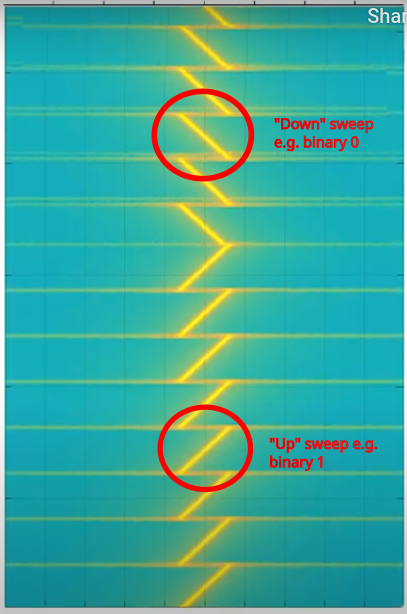
\includegraphics[width=0.5\textwidth]{images/chirp_spread_spectrum_labeled}
\caption{Example of a chirp spread spectrum transmission, highlighting the up and down sweeps which represent binary 1 and 0. \cite{Wenner2017_hd}}
\label{fig:chirp_spread_spectrum_labeled}
\end{figure}

Figure \ref{fig:chirp_spread_spectrum_labeled} provides a visual representation of the chirp spread spectrum technology. This technique encodes data in the frequency variation of the signals over time. A "chirp" refers to a timeframe of the signal where the frequency is increasing or decreasing within a certain bandwidth. This technique makes the signal significantly more resistant to interference compared to simply having two distinct frequencies which are pre-defined to represent a binary 0 or 1, and simply switching between them when transmitting the signal, an example of which can be seen in figure \ref{fig:frequency_shift_keying_labeled}. The up and down sweeps in figure \ref{fig:chirp_spread_spectrum_labeled} visually reflect the bitstream and how it is encoded into radio frequencies.

\begin{figure}[H]
\centering
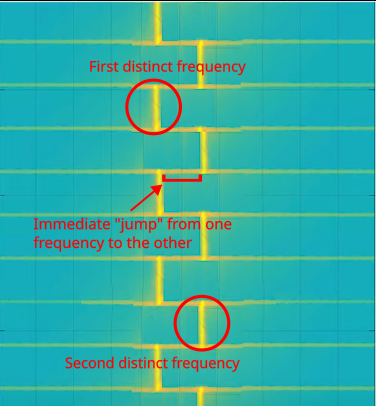
\includegraphics[width=0.5\textwidth]{images/frequency_shift_keying_labeled.png}
\caption{Example of having two distinct frequencies representing binary 0 and 1, and "jumping" between them instead of sweeping. \cite{Wenner2017_hd}}
\label{fig:frequency_shift_keying_labeled}
\end{figure}

Each character transmitted with LoRa lasts a duration determined by the spreading factor, defining how long each chirp lasts. As spreading factor increases, chirps last longer and have improved sensitivity at the expense of having a lower data transmission rate.

LoRaWAN builds upon the LoRa physical layer by adding a media access control (MAC) protocol. It defines how devices connect, how data is encrypted, and how the network is managed. LoRaWAN is designed for ultra-low-power operations, allowing devices to last several years on small batteries, and offers deep indoor penetration, which is particularly valuable in hospital settings where walls and medical equipment can attenuate signals \cite{lora_documentation}.

To assess the suitability of LoRaWAN, it is important to compare it to other LPWAN technologies, including SigFox, NB-IoT, and LTE-M.

SigFox is a proprietary ultra-narrowband communication technology designed for transmitting small data payloads over long distances, while consuming small amounts of power. It operates on unlicensed Industrial, Scientific, and Medical (ISM) bands, and works best when the application requries one-way, infrequent transmissions. These attributes make it great for low-throughput applications, such as smart city metering, and environmental monitoring. Due to some issues with non-fixed environments such as frequency inaccuracies and interference, SigFox works best when employed in fixed locations \cite{sigfox_advantages_disadvantages}.

NB-IoT on the other hand operates in the licensed spectrum. Developed by 3GPP, it offers powerful indoor penetration, is reliable, and allows for connecting a large number of devices. It is mainly suited for applications needing regular (unlike SigFox), low data rate communication, like utility metering and building automation \cite{nbiot_advantages_disadvantages}.

Once again developed by 3GPP, LTE-M supports higher data rates than NB-IoT and allows for voice communication using Voice over Long-Term Evolution (VoLTE). It ensures seamless handover between cell towers, which makes its use cases more dynamic and mobile, such as asset tracking, pet tracking, and point-of-sale devices \cite{ltem_telenor}.

Below is a table summarising their main advantages and disadvantages.

\begin{table}[H]
\centering
\caption{LPWAN technologies - Advantages \& Disadvantages \cite{sigfox_advantages_disadvantages, nbiot_advantages_disadvantages, ltem_advantages_disadvantages, lorawan_advantages_disadvantages}}
\begin{tabularx}{\textwidth}{l X X}
\toprule
\textbf{Technology} & \textbf{Advantages} & \textbf{Disadvantages} \\
\midrule
LoRaWAN &
\begin{itemize}
	\item Long range
	\item Low power consumption
	\item Adaptive data rates
	\item Deep indoor penetration
	\item Low cost
\end{itemize}
&
\begin{itemize}
	\item Limited by duty cycle
	\item Unsuitable for real-time or low latency applications
\end{itemize}
\\
SigFox &
\begin{itemize}
	\item Lightweight protocol
	\item Minimal overhead
	\item Long battery life
	\item Wide coverage
	\item Underground support
\end{itemize}
&
\begin{itemize}
	\item One-way communication
	\item Limited data rates
	\item One operator per country
\end{itemize}
\\
NB-IoT &
\begin{itemize}
	\item High scalability
	\item Robust QoS
	\item Extended range
	\item Structure penetration
	\item Backed by operators
\end{itemize}
&
\begin{itemize}
	\item Licensed spectrum costs
	\item Lower data rates than LTE-M
	\item No roaming support
\end{itemize}
\\
LTE-M &
\begin{itemize}
	\item High data rates
	\item Excellent coverage
	\item LTE network integration
	\item Efficient power use
\end{itemize}
&
\begin{itemize}
	\item Higher costs
	\item Firmware updates consume power
	\item Not for high-volume data
\end{itemize}
\\
\bottomrule
\end{tabularx}
\label{tab:lpwan_adv_disadv}
\end{table}



Bluetooth is also widely used in medical IoT devices. While it offers short-range connectivity and is well-suited for personal health devices like heart rate monitors and themometers, its power consumption and range limit its usefulness for hospital-wide or remote patient monitoring. Bluetooth Low Energy (BLE) improves power efficiency and is increasingly integrated into wearable medical devices. As such, it will be used in this project to connect the main system with the medical sensors which take actual readings.

\subsubsection{Testing}
While the focus of this project was not to benchmark the LoRaWAN protocol itself, preliminary simulations were conducted to validate its suitability for post-operative monitoring applications. A single base station scenario was simulated using open-source software provided by Lancaster University \cite{lancaster_uk_simulation_software}. The simulation was adapted to run on Python 3, and tests were conducted with 100 to 1000 node configurations, increasing by 100 each experiment. The parameters for the simulations where fixed as such: \texttt{AVGSEND = 100ms}, \texttt{SIMTIME = 2000ms}, and \texttt{COLLISION = 1} to enable full collision detection. The parameters used correspond to the simulated nodes transmitting small packets roughly every 100 milliseconds over a total simulation time of two seconds. Furthermore, \texttt{EXPERIMENT = 0} was used, which configures all nodes to transmit with the slowest LoRa modulation settings. The key objective was to confirm that LoRaWAN could handle multiple nodes transmitting small amounts of data at low power over long distances.

\vspace{1em} \noindent The first set of results explore how node density affects transmission quality:
\begin{figure}[H]
\centering
\begin{subfigure}{0.48\textwidth}
	\centering
	\begin{tikzpicture}
\begin{axis}[
	width=\textwidth,
	height=6cm,
	grid=both,
	xlabel={Number of Nodes},
	ylabel={Number of Collisions},
	title={Collisions vs Number of Nodes},
	tick label style={font=\small},
	label style={font=\small},
	title style={font=\small}
]
\addplot[
	color=orange,
	mark=*,
	thick
] table [x=Nodes, y=Collisions, col sep=comma] {graphs/collisions_vs_nodes_all.csv};
\end{axis}
\end{tikzpicture}

	\caption{Collisions vs Number of Nodes}
	\label{fig:collisions_vs_nodes}
\end{subfigure}
\hfill
\begin{subfigure}{0.48\textwidth}
	\centering
	\begin{tikzpicture}
\begin{axis}[
	width=\textwidth,
	height=6cm,
	grid=both,
	xlabel={Number of Nodes},
	ylabel={Transmissions per Node},
	title={Transmission Efficiency vs Number of Nodes},
	tick label style={font=\small},
	label style={font=\small},
	title style={font=\small}
]
\addplot[
	only marks,
	color=teal,
	mark=*,
	% thick
	mark options={scale=1}
] table [x=Nodes, y=Efficiency, col sep=comma] {graphs/efficiency_vs_nodes_all.csv};
\end{axis}
\end{tikzpicture}

	\caption{Transmission Efficiency per Node}
	\label{fig:efficiency_vs_nodes}
\end{subfigure}
\caption{Impact of node count on number of collisions and transmission efficiency.}
\end{figure}

As per Figure \ref{fig:collisions_vs_nodes} the number of collisions increases with the number of nodes linearly, something that is consistent with LoRaWAN's unslotted ALOHA-based access scheme. Regardless, transmission efficiency (Figure \ref{fig:efficiency_vs_nodes}) remained relatively stable, even if it did drop slightly around the 500 node point. This demonstrates LoRaWAN's robustness even under increased load.

\vspace{1em} \noindent The next two plots look at power efficiency against the number of nodes, and the physical spatial distribution of the simulated nodes.

\begin{figure}[H]
\centering
\begin{subfigure}{0.48\textwidth}
	\centering
	\begin{tikzpicture}
\begin{axis}[
	width=\textwidth,
	height=6cm,
	grid=both,
	xlabel={Number of Nodes},
	ylabel={Energy Consumption},
	title={Energy Consumption vs Number of Nodes},
	tick label style={font=\small},
	label style={font=\small},
	title style={font=\small}
]
\addplot[
	color=purple,
	mark=*,
	thick
] table [x=Nodes, y=Energy, col sep=comma] {graphs/energy_vs_nodes_all.csv};
\end{axis}
\end{tikzpicture}

	\caption{Energy Consumption vs Number of Nodes}
	\label{fig:energy_vs_nodes}
\end{subfigure}
\hfill
\begin{subfigure}{0.48\textwidth}
	\centering
	\begin{tikzpicture}
\begin{axis}[
	width=\textwidth,
	height=6cm,
	grid=both,
	xlabel={X Coordinate},
	ylabel={Y Coordinate},
	title={Spatial Distribution of Nodes},
	axis equal
]
\addplot[
	only marks,
	mark=*,
	color=red,
	mark size=1pt
] table [x=X, y=Y, col sep=comma] {graphs/spatial_distribution_all.csv};
\end{axis}
\end{tikzpicture}

	\caption{Spatial Distribution of Nodes}
	\label{fig:spatial_distribution}
\end{subfigure}
\caption{Energy scalability and simulation topology.}
\end{figure}

Figure \ref{fig:energy_vs_nodes} shows that energy consumption of each node scaled linearly once more with the number of nodes. This is to be expected as all nodes use the same transmit settings and a fixed sending interval. Provided duty cycles are properly managed, these results support LoRaWAN's use in battery-powered applications. A duty cycle is the time a device is permitted to transmit on a given frequency band, within a set time period \cite{duty_cycles}. The spatial distribution (Figure \ref{fig:spatial_distribution}) simply confirms that the simulation used a random deployment of the nodes across the simulated physical area, approximating a real-world environment such as a hospital ward.

\vspace{1em} \noindent Path loss and signal strength trends were also considered to better understand signal behaviour.
\begin{figure}[H]
\centering
\begin{subfigure}{0.48\textwidth}
	\centering
	\centering
\begin{tikzpicture}
\begin{axis}[
	width=\textwidth,
	height=6cm,
	grid=both,
	xlabel={Distance (m)},
	ylabel={RSSI (dBm)},
	title={RSSI vs Distance}
]
\addplot[
	only marks,
	mark=*,
	color=blue,
	mark size=1pt
] table [x=Distance, y=RSSI, col sep=comma] {graphs/rssi_vs_distance_all.csv};
\end{axis}
\end{tikzpicture}
\caption{RSSI values relative to distance from the gateway.}

	\caption{RSSI vs Distance}
	\label{fig:rssi_vs_distance}
\end{subfigure}
\hfill
\begin{subfigure}{0.48\textwidth}
	\centering
	\centering
\begin{tikzpicture}
\begin{axis}[
	width=\textwidth,
	height=6cm,
	grid=both,
	xlabel={Distance (m)},
	ylabel={Lpl (dB)},
	title={Lpl vs Distance},
	tick label style={font=\small},
	label style={font=\small},
	title style={font=\small},
]
\addplot[
	only marks,
	mark=*,
	color=green,
	mark size=1pt
] table [x=Distance, y=Lpl, col sep=comma] {graphs/lpl_vs_distance_all.csv};
\end{axis}
\end{tikzpicture}
	\caption{Path loss (Lpl) values relative to node distance from the gateway.}

	\caption{Path Loss (Lpl) vs Distance}
	\label{fig:lpl_vs_distance}
\end{subfigure}
\caption{Signal strength and path loss trends relative to node distance from the gateway}
\end{figure}

Both path loss and Received Signal Strength Index (RSSI) degrade as the distance increases, which is to be expected based on theoretical radio propagation models. RSSI is a representation of the measurement of power level for a received radio signal. It is typically expressed in dBm, and as the values get more negative, it indicates a weaker signal.

Results showed that as the number of nodes doubled, the number of collisions also increased, which is consistent with LoRaWAN's access behaviour. In this context, a \textit{collision} refers to the event where multiple decvices transmit at the same time, on the same frequency, and with the same spreading factor, at overlapping times, leading to signal interference at the gateway. When collisions occur, the gateway will likely have trouble demodulating the incoming transmitted packets, causing data loss.

Despite the increase in collisions, transmission efficiency per node remained stable, and energy consumption scaled predictably with the node count --- highlighting LoRaWAN's suitability for applications requiring scalability, wide coverage, and energy efficiency, such as this project. Compared to Wi-Fi, LoRaWAN uses significantly less power and has a vastly longer communication range. Wi-Fi needs to have constant connectivity, and frequently send beacons out informing end devices of available access points and services \cite{wifi_beacons}. These two facts mean Wi-Fi consumes substantially more power than LoRaWAN making it unsuitable for battery operated devices intended for long-term use (in the order of years). Furthermore, Wi-Fi was designed for high-throughput applications in a limited range in indoor environments, unlike LoRaWAN which was designed for sparse, low data rate transmission covering large areas. As for GSM-based technologies like NB-IoT and LTE-M, while they do offer broader coverage and existing infrastructure backed and maintained by mobile providers, they come with significantly higher costs, greater power needs, and licensing requirements (meaning legally only mobile network operators can operate them, or a partnership with a mobile operator is requried), making them not as suitable for this application as LoRaWAN is. The comparison in Table \ref{tab:lpwan_adv_disadv} illustrates the advantages of LoRaWAN in terms of its efficient power consumption, cost, and flexibility in deployment and operation.

These outcomes support the choice of LoRaWAN as a communication backbone in the system, balancing scalability and energy efficiency in a medical monitoring context.

\section{Commercially available medical devices} % Section 2.5
Because Bluetooth technology combined with technologies allowing integration with the cloud allow for continuous, real-time monitoring of vital signs including heart rate, blood pressure, respiration rate, temperature, and oxygen saturation, they have completely changed postoperative treatment. Such devices enable smooth data transfer to medical professionals, enabling prompt interventions and individualised patient treatment. Numerous Bluetooth-enabled medical devices are available on the market, with differences in performance, compatibility, and data access transparency. Since it dictates how easily these devices may be integrated with other healthcare systems and apps such as the one discussed in this thesis, the level of Bluetooth openness is especially important. I will examine a number of commercially available devices that demonstrate these characteristics in the sections that follow, emphasising their features and clinical application considerations.

Numerous commercially available medical devices can be used in clinical settings and are made for the continuous monitoring of vital signs. Selected devices are summarised in the table below, with an emphasis on those that have been certified for clinical use by the US Food and Drug Administration (FDA) or that bear the CE mark in accordance with the EU Medical Device Regulation. It is important to keep in mind that FDA approval entails a more stringent examination procedure and is frequently thought of as a higher quality of clinical validation, even if the CE mark certifies regulatory conformity.

The table features the certification granted to the device, the measured vital signs, and its Bluetooth openness level. Each device listed is capable of measuring one or more of the following vital signs:

\begin{itemize}
			\item \textbf{HR:} Heart Rate
			\item \textbf{BP:} Blood Pressure (may be traditional or cuffless)
			\item \textbf{RR:} Respiratory Rate
			\item \textbf{SpO\textsubscript{\textbf{2}}:} Blood Oxygen Saturation
			\item \textbf{Temp:} Body Temperature
			\item \textbf{ECG:} Electrocardiogram
\end{itemize}

The term "Bluetooth openness" indicates how simple it is to access and incorporate data into customised solutions. Interoperability may be a constraint for customised IoT solutions because the majority of clinically certified devices function within proprietary ecosystems.

\begin{table}[H]
\centering
\caption{Medically Certified Bluetooth Capable Devices}
	\renewcommand{\arraystretch}{1.2}
	\begin{tabularx}{\textwidth}{|>{\RaggedRight\arraybackslash}X|>{\RaggedRight\arraybackslash}X|>{\RaggedRight\arraybackslash}X|>{\RaggedRight\arraybackslash}X|>{\RaggedRight\arraybackslash}X|}
	\hline
	\textbf{Device Name} & \textbf{Manufacturer} & \textbf{Certification} & \textbf{Vital Signs it Measures} & \textbf{Bluetooth Openness} \\
	\hline
	GE Portrait Mobile & GE HealthCare & FDA & HR, RR, SpO$_2$, Temp & Closed \\ 
	\hline
	Berry Multi-Parameter Monitor & Berry Medical & CE (MDR) & HR, BP, SpO$_2$, Temp, ECG & Semi-open \\
	\hline
		Contec CMS8000 & Contec Medical & CE (MDR) & HR, BP, SpO$_2$, Temp, RR, ECG & Closed \\
		\hline
		Biobeat Chest Patch & Biobeat & FDA, CE (MDR) & HR, BP (cuffless), SpO$_2$, RR, Temp & Closed \\
		\hline
		Caretaker4 & Caretaker Medical & CE (MDR) & BP, HR, RR, SpO$_2$ & Closed \\
		\hline
		Checkme Pro Vital Signs Monitor & Wellue (Viatom) & CE (MDR) & HR, BP, SpO$_2$, Temp, ECG & Semi-open \\
		\hline
		CardiacSense Watch & CardiacSense & CE (MDR) & HR, ECG, SpO$_2$, Temp & Closed \\
		\hline
		SIFVITAL-1.2 & SIFSOF & CE (MDR) & HR, BP, SpO$_2$, Temp, Glucose & Closed \\
		\hline
		CARER HC-03 6-in-1 Monitor & CARER Medical & CE (MDR) & HR, BP, SpO$_2$, Temp, Glucose, ECG & Closed \\
		\hline
		Lepu Vital Signs Monitor & Lepu Medical & CE (MDR) & HR, BP, SpO$_2$, Temp, ECG & Closed \\
		\hline
	\end{tabularx}
	\renewcommand{\arraystretch}{1.0}
\label{tab:lpwan_adv_disadv}
\end{table}



Even though a lot of devices fulfil the requirements for medical certification, as the table shows, they frequently lack open Bluetooth interfaces. When incorporating them into custom IoT systems, this poses a problem, which will be discussed in the next section along with suggestions for dealing with it.

\section{Integration with custom IoT systems} % Section 2.6
Because of the restricted or proprietary nature of their Bluetooth communication protocols, it is still very difficult to integrate commercially available vital signs monitors into custom Internet of Things (IoT) systems. As mentioned in the preceding section, the majority of devices offer little to no support for open data access, despite the fact that many of them are medically certified and give accurate physiological readings. Some, at most, provide semi-open APIs that are restricted to partner software or vendor-specific apps. This makes it more difficult to integrate seamlessly with specially designed systems that seek to independently gather, process, or send data. The impacts of these restrictions are examined in this section, along with possible interoperability tactics for medical IoT applications.

\subsubsection{Challenges and Implications}
Even though there are medically recognised vital sign measurement devices available, Bluetooth accessibility issues make it difficult to integrate them into custom IoT systems. The majority of medical equipment intended for professional usage rely on closed data ecosystems or proprietary Bluetooth protocols. The functionality is frequently confined to vendor-approved apps or limited APIs, preventing complete integration with customised microcontroller-based systems, even in situations where some Bluetooth access is offered.

This lack of openness presents a number of practical and technical difficulties. First, there are significant limitations on compatibility. Raw vital sign data cannot be directly accessed by custom systems that depend on local gateways or lightweight edge devices (like Arduino or ESP32) unless the device supports standard Bluetooth Generic Attribute Profile (GATT) profiles or offers a published Application Programming Interface (API). Consequently, the two main advantages of edge-based IoT architectures—real-time processing and on-device decision-making—become impracticable. Second, vendor lock-in develops into an extremely serious issue. System designers are left with no control over data flow, privacy policies, and long-term data preservation when device data is only available via the cloud platforms or mobile apps of the manufacturer, which almost certainly makes it more difficult to comply with data protection laws like GDPR or HIPAA in clinical or research settings where data sovereignty, repeatability, and traceability are crucial.

Furthermore, development time and integration complexity also rise. Reverse engineering, unapproved Software Development Kits (SDKs), or intricate workarounds are frequently required in order to retrieve useful data from these devices. These endeavours are laborious, prone to mistakes, and possibly fragile, as they can fail with firmware changes or violate license agreements.

These difficulties show how the requirements for adaptable, responsive IoT-based monitoring solutions differ from those of authorised commercial devices. To overcome these constraints while maintaining system dependability and regulatory compliance, potential workarounds and integration techniques are examined in the immediately following paragraphs.

\subsubsection{Possible Solutions}
Developers of custom IoT systems must think of alternate ways to enable integration while preserving clinical dependability and compliance, given the limitations imposed by proprietary Bluetooth implementations in medically approved vital sign monitors. While there isn't a single solution that works for all, there are a few workarounds that could enable significant interoperability despite the existing constraints.

\begin{enumerate}
	\item \textbf{Use of intermediate devices with vendor APIs}
	\item[] Data can be accessed by official desktop software or mobile applications in certain closed systems. In these situations, middleware bridges that communicate with the vendor software through open SDKs or REST APIs can be created, such as companion Raspberry Pi services or smartphone apps. These intermediary devices can then use standardised protocols to send the necessary information to customised IoT devices. This maintains data accuracy and honours the device's intended usage paradigm, even if it adds another layer of complexity and can cause latency to increase.
	\item \textbf{Preferring semi-open devices to entirely closed devices}
	\item[] Vendors occasionally offer limited Bluetooth access via documented GATT profiles or custom services. Although they are not completely open, devices like the Wellue Checkme Pro provide restricted data access that can be adequate for everyday uses. When feasible, system designers should give priority to these semi-open devices and use reverse-engineered documentation or community-developed libraries to retrieve readings with the least amount of intrusion to prevent any legal problems regarding licensing agreements.
	\item \textbf{Passive signal interception (may violate licensing agreements)}
	\item[] Certain specialised tools can be used to determine the transmission structure of the Bluetooth signals sent from closed sensor devices, and reverse-engineer the communication protocol in devices without access to an API or access point. Although this method can provide complete access to sensor data, it is not recommended for production systems or environments that need to adhere to legal or clinical requirements since it runs the risk of breaking user agreements and regulatory restrictions.
	\item \textbf{Develop sensor systems in parallel}
	\item[] By constructing parallel sensor modules with clinically proven open hardware or certified discrete sensors (e.g., MAX30101 for SpO$_2$ and pulse, MLX90614 for temperature), it is also possible to entirely eliminate reliance on closed devices. This provides complete firmware-level control over sensing, communication, and data handling, but it is more taxing in terms of development resources. Full-stack customisation is made possible by the direct integration of such customised sensors with system infrastructure when paired with LoRa, BLE, or Wi-Fi transmission modules.
	\item \textbf{Collaboration with vendors and enterprise partnerships}
	\item [] Organisations can contact vendors for OEM agreements or developer access when commercial devices are preferred. On request, certain manufacturers might provide enterprise SDKs or documentation, particularly for system integration pilot programs, academic research, or clinical trials. Even though it could take more time, this approach guarantees long-term support and compliance.
	\item[] The expense, complexity, and legality of each of these workarounds are trade-offs. The best strategy frequently calls for a hybrid system, in which open or semi-open alternatives are utilised for system development or simulation, while medically certified but closed devices are utilised for clinical validation. In the end, market forces and regulatory pressure may push manufacturers towards greater openness in upcoming device generations as the need for patient-specific, interoperable healthcare systems increases.
\end{enumerate}

\section{Summary} % Section 2.7
There are technological and legal issues with integrating medically approved vital sign monitoring devices into unique IoT systems. Even if a lot of commercial devices provide precise and trustworthy measurements, smooth integration is hampered by their closed or semi-open Bluetooth implementations, which restrict direct access to raw data streams. These restrictions may affect custom healthcare platforms' adaptability, reactivity, and independence. However, there are a number of practical alternatives, such as using semi-open devices, developing parallel sensing modules, using middleware programs, or forming direct relationships with manufacturers. For IoT healthcare solutions to be scalable, interoperable, and patient-tailored, these integration hurdles must be removed.
